% Options for packages loaded elsewhere
% Options for packages loaded elsewhere
\PassOptionsToPackage{unicode}{hyperref}
\PassOptionsToPackage{hyphens}{url}
\PassOptionsToPackage{dvipsnames,svgnames,x11names}{xcolor}
%
\documentclass[
  13pt,
]{article}
\usepackage{xcolor}
\usepackage[margin=2cm]{geometry}
\usepackage{amsmath,amssymb}
\setcounter{secnumdepth}{5}
\usepackage{iftex}
\ifPDFTeX
  \usepackage[T1]{fontenc}
  \usepackage[utf8]{inputenc}
  \usepackage{textcomp} % provide euro and other symbols
\else % if luatex or xetex
  \usepackage{unicode-math} % this also loads fontspec
  \defaultfontfeatures{Scale=MatchLowercase}
  \defaultfontfeatures[\rmfamily]{Ligatures=TeX,Scale=1}
\fi
\usepackage{lmodern}
\ifPDFTeX\else
  % xetex/luatex font selection
  \setmainfont[]{Times New Roman}
\fi
% Use upquote if available, for straight quotes in verbatim environments
\IfFileExists{upquote.sty}{\usepackage{upquote}}{}
\IfFileExists{microtype.sty}{% use microtype if available
  \usepackage[]{microtype}
  \UseMicrotypeSet[protrusion]{basicmath} % disable protrusion for tt fonts
}{}
\usepackage{setspace}
\makeatletter
\@ifundefined{KOMAClassName}{% if non-KOMA class
  \IfFileExists{parskip.sty}{%
    \usepackage{parskip}
  }{% else
    \setlength{\parindent}{0pt}
    \setlength{\parskip}{6pt plus 2pt minus 1pt}}
}{% if KOMA class
  \KOMAoptions{parskip=half}}
\makeatother
% Make \paragraph and \subparagraph free-standing
\makeatletter
\ifx\paragraph\undefined\else
  \let\oldparagraph\paragraph
  \renewcommand{\paragraph}{
    \@ifstar
      \xxxParagraphStar
      \xxxParagraphNoStar
  }
  \newcommand{\xxxParagraphStar}[1]{\oldparagraph*{#1}\mbox{}}
  \newcommand{\xxxParagraphNoStar}[1]{\oldparagraph{#1}\mbox{}}
\fi
\ifx\subparagraph\undefined\else
  \let\oldsubparagraph\subparagraph
  \renewcommand{\subparagraph}{
    \@ifstar
      \xxxSubParagraphStar
      \xxxSubParagraphNoStar
  }
  \newcommand{\xxxSubParagraphStar}[1]{\oldsubparagraph*{#1}\mbox{}}
  \newcommand{\xxxSubParagraphNoStar}[1]{\oldsubparagraph{#1}\mbox{}}
\fi
\makeatother


\usepackage{longtable,booktabs,array}
\usepackage{calc} % for calculating minipage widths
% Correct order of tables after \paragraph or \subparagraph
\usepackage{etoolbox}
\makeatletter
\patchcmd\longtable{\par}{\if@noskipsec\mbox{}\fi\par}{}{}
\makeatother
% Allow footnotes in longtable head/foot
\IfFileExists{footnotehyper.sty}{\usepackage{footnotehyper}}{\usepackage{footnote}}
\makesavenoteenv{longtable}
\usepackage{graphicx}
\makeatletter
\newsavebox\pandoc@box
\newcommand*\pandocbounded[1]{% scales image to fit in text height/width
  \sbox\pandoc@box{#1}%
  \Gscale@div\@tempa{\textheight}{\dimexpr\ht\pandoc@box+\dp\pandoc@box\relax}%
  \Gscale@div\@tempb{\linewidth}{\wd\pandoc@box}%
  \ifdim\@tempb\p@<\@tempa\p@\let\@tempa\@tempb\fi% select the smaller of both
  \ifdim\@tempa\p@<\p@\scalebox{\@tempa}{\usebox\pandoc@box}%
  \else\usebox{\pandoc@box}%
  \fi%
}
% Set default figure placement to htbp
\def\fps@figure{htbp}
\makeatother


% definitions for citeproc citations
\NewDocumentCommand\citeproctext{}{}
\NewDocumentCommand\citeproc{mm}{%
  \begingroup\def\citeproctext{#2}\cite{#1}\endgroup}
\makeatletter
 % allow citations to break across lines
 \let\@cite@ofmt\@firstofone
 % avoid brackets around text for \cite:
 \def\@biblabel#1{}
 \def\@cite#1#2{{#1\if@tempswa , #2\fi}}
\makeatother
\newlength{\cslhangindent}
\setlength{\cslhangindent}{1.5em}
\newlength{\csllabelwidth}
\setlength{\csllabelwidth}{3em}
\newenvironment{CSLReferences}[2] % #1 hanging-indent, #2 entry-spacing
 {\begin{list}{}{%
  \setlength{\itemindent}{0pt}
  \setlength{\leftmargin}{0pt}
  \setlength{\parsep}{0pt}
  % turn on hanging indent if param 1 is 1
  \ifodd #1
   \setlength{\leftmargin}{\cslhangindent}
   \setlength{\itemindent}{-1\cslhangindent}
  \fi
  % set entry spacing
  \setlength{\itemsep}{#2\baselineskip}}}
 {\end{list}}
\usepackage{calc}
\newcommand{\CSLBlock}[1]{\hfill\break\parbox[t]{\linewidth}{\strut\ignorespaces#1\strut}}
\newcommand{\CSLLeftMargin}[1]{\parbox[t]{\csllabelwidth}{\strut#1\strut}}
\newcommand{\CSLRightInline}[1]{\parbox[t]{\linewidth - \csllabelwidth}{\strut#1\strut}}
\newcommand{\CSLIndent}[1]{\hspace{\cslhangindent}#1}



\setlength{\emergencystretch}{3em} % prevent overfull lines

\providecommand{\tightlist}{%
  \setlength{\itemsep}{0pt}\setlength{\parskip}{0pt}}



 


\usepackage{booktabs}
\usepackage{longtable}
\usepackage{array}
\usepackage{multirow}
\usepackage{wrapfig}
\usepackage{float}
\usepackage{colortbl}
\usepackage{pdflscape}
\usepackage{tabu}
\usepackage{threeparttable}
\usepackage{threeparttablex}
\usepackage[normalem]{ulem}
\usepackage{makecell}
\usepackage{xcolor}
\usepackage[noblocks]{authblk}
\renewcommand*{\Authsep}{, }
\renewcommand*{\Authand}{, }
\renewcommand*{\Authands}{, }
\renewcommand\Affilfont{\small}
\makeatletter
\@ifpackageloaded{caption}{}{\usepackage{caption}}
\AtBeginDocument{%
\ifdefined\contentsname
  \renewcommand*\contentsname{Table of contents}
\else
  \newcommand\contentsname{Table of contents}
\fi
\ifdefined\listfigurename
  \renewcommand*\listfigurename{List of Figures}
\else
  \newcommand\listfigurename{List of Figures}
\fi
\ifdefined\listtablename
  \renewcommand*\listtablename{List of Tables}
\else
  \newcommand\listtablename{List of Tables}
\fi
\ifdefined\figurename
  \renewcommand*\figurename{Figure}
\else
  \newcommand\figurename{Figure}
\fi
\ifdefined\tablename
  \renewcommand*\tablename{Table}
\else
  \newcommand\tablename{Table}
\fi
}
\@ifpackageloaded{float}{}{\usepackage{float}}
\floatstyle{ruled}
\@ifundefined{c@chapter}{\newfloat{codelisting}{h}{lop}}{\newfloat{codelisting}{h}{lop}[chapter]}
\floatname{codelisting}{Listing}
\newcommand*\listoflistings{\listof{codelisting}{List of Listings}}
\makeatother
\makeatletter
\makeatother
\makeatletter
\@ifpackageloaded{caption}{}{\usepackage{caption}}
\@ifpackageloaded{subcaption}{}{\usepackage{subcaption}}
\makeatother
\usepackage{bookmark}
\IfFileExists{xurl.sty}{\usepackage{xurl}}{} % add URL line breaks if available
\urlstyle{same}
\hypersetup{
  pdftitle={Changes in meritocratic beliefs among school-age students over time and across cohorts},
  colorlinks=true,
  linkcolor={blue},
  filecolor={Maroon},
  citecolor={Blue},
  urlcolor={Blue},
  pdfcreator={LaTeX via pandoc}}


\title{Changes in meritocratic beliefs among school-age students over
time and across cohorts}



\date{}
\begin{document}
\maketitle
\begin{abstract}
Besides transmitting academic knowledge, schools are key sites of
meritocratic socialization, actively shaping students' understanding of
whether success is earned or inherited. Yet the measurement of students'
meritocratic beliefs remains underdeveloped: most instruments conflate
perceptions of how rewards are allocated with normative preferences for
how they should be allocated, and treat merit and privilege as mutually
exclusive. This study tests a multidimensional model that distinguishes
four dimensions among school-aged students: perceived meritocracy and
meritocratic preferences (whether effort and talent are, and should be,
rewarded), and perceived privilege and privilege acceptance (whether
family wealth and connections shape outcomes, and whether this is seen
as legitimate). Using two-wave panel survey data from Chilean students
in 8th and 10th grade (Wave 1: N = 846; Wave 2: N = 662), we assess
whether these dimensions can be distinguished, compared across school
stages, and measured equivalently over time using confirmatory factor
analysis and measurement invariance testing. Results support a
four-factor structure, showing that endorsement of merit coexists with
recognition of privilege rather than displacing it. The scale achieves
strict longitudinal invariance within students, enabling valid
developmental comparisons, but not across school levels, indicating that
older students apply a more critical frame when judging whether effort
is rewarded. These findings provide a validated instrument for tracking
how meritocratic beliefs develop through schooling. They are relevant
for civic education, school climate, and equity-oriented policy, where
students' sense of fairness is central: because students can demand
merit-based fairness precisely when they perceive its absence,
interpreting their beliefs requires distinguishing what students
perceive from what they endorse, and merit from privilege, rather than
treating belief in meritocracy as a single attitude to reinforce or
counter. \newline \textbf{Keywords}: Meritocracy · Schools · Measurement
invariance · Socialization · Chile
\end{abstract}


\setstretch{1.5}
\section{Introduction}\label{introduction}

How students come to understand who succeeds and why is one of the
central questions in sociology of education
(\citeproc{ref-mijs_unfulfillable_2016}{Mijs, 2016};
\citeproc{ref-resh_sense_2014}{Resh \& Sabbagh, 2014}). Schools are
central sites in this process: they simultaneously promote meritocracy
as a cultural ideal, presenting education as the legitimate route to
upward mobility and individual effort as the proper basis of social
rewards (\citeproc{ref-vandewerfhorst_meritocracy_2024}{Van De
Werfhorst, 2024}), and institutionalize it as a lived experience through
grading, tracking, and selection
(\citeproc{ref-darnon_where_2018}{Darnon, Wiederkehr, et al., 2018};
\citeproc{ref-traini_stratification_2022}{Traini, 2022}). Students who
believe that effort and talent determine outcomes tend to interpret
success and failure in individual terms, with consequences that extend
from individual motivation to school climate and beliefs about social
inequality (\citeproc{ref-castillo_socialization_2024}{Castillo et al.,
2024}; \citeproc{ref-resh_sense_2018a}{Resh, 2018};
\citeproc{ref-weinberg_countrylevel_2021}{Weinberg et al., 2021}). Yet
students also encounter daily evidence that outcomes are shaped by
family background, social connections, and structural advantage,
creating tensions between meritocratic ideals and lived experience
(\citeproc{ref-bourdieu_reproduction_1990}{Bourdieu \& Passeron, 1990};
\citeproc{ref-goudeau_hidden_2017a}{Goudeau \& Croizet, 2017};
\citeproc{ref-tang_meritocratic_2025}{Tang et al., 2025}). Understanding
how students hold these beliefs, whether they see society as
meritocratic, whether they think it should be, and whether these
judgments extend to privilege, is therefore a question with direct
relevance for educational practice and equity in schools.

What makes this particularly complex is that students rarely hold these
beliefs in pure form. Meritocratic beliefs carry concrete educational
consequences: among teachers, belief in school meritocracy predicts
preference for competitive over cooperative classroom practices; among
parents, lower demand for equity-oriented policies; and among students,
reduced support for interventions aimed at reducing achievement gaps and
stronger legitimation of inequality
(\citeproc{ref-batruch_belief_2022}{Batruch et al., 2022};
\citeproc{ref-castillo_socialization_2024}{Castillo et al., 2024};
\citeproc{ref-darnon_competitive_2023}{Darnon et al., 2023};
\citeproc{ref-darnon_where_2018}{Darnon, Wiederkehr, et al., 2018};
\citeproc{ref-wiederkehr_belief_2015}{Wiederkehr et al., 2015}).
However, even students who recognize that family wealth and connections
shape outcomes may simultaneously endorse meritocracy as a normative
ideal, reflecting what the literature describes as dual consciousness
(\citeproc{ref-liu_does_2025}{C. Liu \& Wang, 2025};
\citeproc{ref-tang_meritocratic_2025}{Tang et al., 2025}). Whether and
how the consequences above differ depending on whether students are
expressing perceptions or preferences, and about merit or privilege, is
precisely what current research has rarely been able to establish.

Despite this complexity, the field lacks adequate tools to capture these
distinctions. Most instruments conflate what students perceive to be
true about how rewards are distributed with what they prefer should be
true, and treat merit and privilege as opposite ends of a single scale.
A student who perceives that only connections and wealth get ahead but
strongly believes that effort and talent should determine outcomes holds
a fundamentally different orientation from a student who is indifferent
to both, yet current instruments would assign them similar scores,
misidentifying what students believe and what educational responses
should address.

This study addresses this gap with two contributions to educational
research. The first is the validation of a multidimensional model of
meritocratic beliefs for school-aged populations, building on Castillo
et al.'s (\citeproc{ref-castillo_multidimensional_2023}{2023})
framework, which distinguishes between perceptions of how meritocracy
operates (``what is'') and preferences about how it should (``what ought
to be''), and between meritocratic elements (effort, talent) and
privilege-based elements (family wealth, personal contacts). Treating
these as four distinct but related dimensions, rather than collapsing
them into a single score or a bipolar scale
(\citeproc{ref-reynolds_perceptions_2014a}{Reynolds \& Xian, 2014}),
allows for belief profiles that unidimensional instruments rule out by
design, and provides a stronger empirical basis for studying how schools
shape students' orientations toward fairness and inequality. While
recent work has begun to treat school meritocracy as multidimensional
(\citeproc{ref-chauvin_school_2026}{Chauvin et al., 2026}), no validated
instrument yet captures these distinctions among students themselves, a
gap this study addresses directly.

The second contribution is to examine whether this instrument functions
equivalently across school stages (8th vs.~10th grade) and over time
within the same students (2023-2024). Most research on meritocratic
beliefs remains cross-sectional, limiting what we can infer about how
these orientations develop during adolescence, precisely when reasoning
about justice becomes more sophisticated and school-based sorting
mechanisms grow more salient
(\citeproc{ref-henry_development_2006}{Henry \& Saul, 2006};
\citeproc{ref-resh_sense_2014}{Resh \& Sabbagh, 2014}). Establishing
measurement invariance is a prerequisite for valid developmental
comparisons: without it, observed change over time may reflect shifts in
how students interpret items rather than genuine change in underlying
beliefs (\citeproc{ref-putnick_measurement_2016}{Putnick \& Bornstein,
2016}; \citeproc{ref-vandeschoot_editorial_2015}{Van De Schoot et al.,
2015}). Cross-cohort invariance testing serves a complementary purpose:
rather than assuming comparability across school stages, we treat the
degree of equivalence as an empirical question whose answer is itself
theoretically informative about how educational experience reshapes the
meaning students attach to meritocratic concepts.

This study draws on panel data from Chile, a setting that is both
nationally specific and internationally instructive. Chile's educational
system combines high stratification, market-based competition, and
explicit meritocratic discourse in school culture
(\citeproc{ref-castillo_socialization_2024}{Castillo et al., 2024};
\citeproc{ref-valenzuela_socioeconomic_2013}{Valenzuela et al., 2013}),
alongside persistent socioeconomic inequality and a deep marketization
of social welfare (\citeproc{ref-ferre_welfare_2023}{Ferre, 2023}),
features shared by many Latin American countries and increasingly
present in European and East Asian systems undergoing marketization
(\citeproc{ref-busemeyer_skills_2014}{Busemeyer, 2014};
\citeproc{ref-liu_does_2025}{C. Liu \& Wang, 2025}). This makes Chile a
productive case for studying how students internalize, question, or
reconcile meritocratic ideals with the reality of privilege, while the
dimensional structure and longitudinal patterns identified here are
likely to travel to other highly stratified educational contexts.

The research questions guiding this study are as follows:

\begin{enumerate}
\def\labelenumi{(\arabic{enumi})}
\item
  Do school-aged students distinguish between meritocratic and
  privilege-based principles, as well as between perceptions (``what
  is'') and preferences (``what should be'')?
\item
  Are these dimensions longitudinally stable within students over time,
  and does their measurement equivalence hold across school stages, or
  does educational experience reshape the meaning of meritocratic
  beliefs?
\end{enumerate}

In the following sections, we review the theoretical background on
meritocratic beliefs in school settings, present the methodology and
results, and discuss the implications of our findings for understanding
how meritocratic socialization develops during adolescence and for civic
education, school climate, and equity-oriented policy.

\section{Theoretical and empirical
background}\label{theoretical-and-empirical-background}

\subsection{What is meritocracy and how is it
measured?}\label{what-is-meritocracy-and-how-is-it-measured}

Meritocracy refers to a distributive system in which individual merit,
typically defined as effort and personal ability, is treated as the
primary criterion for allocating resources and rewards, rather than
social origins or inherited privilege
(\citeproc{ref-bell_equality_1972}{Bell, 1972};
\citeproc{ref-young_rise_1958}{Young, 1958}). While Young
(\citeproc{ref-young_rise_1958}{1958}) coined the term as a dystopian
critique, it has since been re-appropriated as a positive ideal of
fairness in liberal and market-oriented societies
(\citeproc{ref-mijs_paradox_2021}{Mijs, 2021};
\citeproc{ref-vandewerfhorst_meritocracy_2024}{Van De Werfhorst, 2024}).
From a sociological standpoint, meritocracy operates both as a cognitive
judgment about how inequality works and as a moral lens through which
people evaluate whether unequal outcomes are deserved
(\citeproc{ref-castillo_meritocracia_2019}{Castillo et al., 2019};
\citeproc{ref-heuer_legitimizing_2020}{Heuer et al., 2020}). Precisely
because it frames outcomes as earned, meritocratic ideals can end up
reinforcing inequality: ``winners'' are encouraged to see their position
as deserved, while ``losers'' are pushed toward self-blame rather than
structural critique
(\citeproc{ref-garcia-sierra_dark_2023}{García-Sierra, 2023};
\citeproc{ref-sandel_tyranny_2020}{Sandel, 2020}). Research in adult
populations has documented systematic associations between these beliefs
and orientations toward redistribution and educational policy
(\citeproc{ref-castillo_perceptions_2025}{Castillo et al., 2025};
\citeproc{ref-tejero-peregrina_perceived_2025}{Tejero-Peregrina et al.,
2025}), but the question of how and when they develop, and whether the
same belief structure emerges among school-aged students who are still
embedded in the socialization processes that shape them, has received
far less attention.

The research agenda on meritocratic beliefs has faced challenges in
conceptualizing and measuring meritocracy. Some studies have relied on
narrow operationalizations that equate meritocracy with the social
valuation of effort (\citeproc{ref-mijs_paradox_2021}{Mijs, 2021};
\citeproc{ref-wiederkehr_belief_2015}{Wiederkehr et al., 2015}), often
reflecting simplified readings of Young's
(\citeproc{ref-young_rise_1958}{1958}) formulation (Merit = Effort +
Intelligence), whereas others treat it as interchangeable with broader
constructs such as system justification
(\citeproc{ref-day_movin_2017}{Day \& Fiske, 2017};
\citeproc{ref-jost_decade_2004a}{Jost et al., 2004}), beliefs about
social mobility (\citeproc{ref-deng_its_2025}{Deng \& Wang, 2025};
\citeproc{ref-mccoy_priming_2007}{McCoy \& Major, 2007}), or generalized
support for equal opportunity
(\citeproc{ref-batruch_belief_2022}{Batruch et al., 2022};
\citeproc{ref-darnon_where_2018}{Darnon, Wiederkehr, et al., 2018}). As
a result, conceptually distinct orientations are frequently collapsed
into a single indicator, and the distinction between descriptive
perceptions of how rewards are allocated and normative preferences about
how they should be allocated is often acknowledged but rarely
implemented analytically.

A related, more specific limitation concerns how studies account for
privilege-based factors such as family wealth, social connections, and
other structural advantages. As Castillo et al.
(\citeproc{ref-castillo_multidimensional_2023}{2023}) notes, much survey
research relies on item batteries that ask respondents to rate the
importance of effort, talent, family background, networks, or luck for
``getting ahead'', and then reduces these into a single score. This
becomes especially problematic when researchers construct difference or
continuum measures, treating meritocratic and privilege-based
explanations as opposite ends of the same scale (e.g., by subtracting
``non-merit'' from ``merit,'' as in
\citeproc{ref-reynolds_perceptions_2014a}{Reynolds \& Xian, 2014}). Such
operationalizations embed a strong zero-sum assumption, namely that
endorsing merit necessarily entails rejecting structural or relational
advantages, thereby ruling out, by design, the empirical possibility
that both types of beliefs coexist. Recent debates, including the
exchange between Mijs (\citeproc{ref-mijs_visualizing_2026}{2026}) and
Wiesner \& Sachweh (\citeproc{ref-wiesner_effort_2026}{2026}),
underscore this point by arguing for measures that capture meritocratic
beliefs alongside privilege-based ones, rather than as a residual of the
relative importance assigned to structural factors. Complementary
empirical work reinforces this concern: meritocratic endorsement can
remain stable even as recognition of structural constraints increases
(\citeproc{ref-liu_does_2025}{C. Liu \& Wang, 2025};
\citeproc{ref-tang_meritocratic_2025}{Tang et al., 2025}), and support
for merit coexists with recognition of social connections rather than
trading off against it
(\citeproc{ref-kwon_multidimensionality_2024}{Kwon \& Pandian, 2024};
\citeproc{ref-zhu_meritocratic_2025}{Zhu, 2025}). Unidimensional
indices, and especially subtraction scores, can therefore manufacture
artificial neutral positions and blur substantively distinct belief
profiles that carry different educational consequences.

In response to these limitations, Castillo et al.
(\citeproc{ref-castillo_multidimensional_2023}{2023}) proposed a
multidimensional framework that decomposes meritocratic beliefs along
two analytically independent axes: preferences versus perceptions, and
meritocratic versus privilege-based allocation principles. Preferences
capture normative ideals about how rewards should be distributed (e.g.,
whether effort and ability ought to determine life chances); perceptions
capture descriptive evaluations of how society actually works (e.g.,
whether observed inequalities reflect merit-based processes)
(\citeproc{ref-janmaat_subjective_2013}{Janmaat, 2013}). Meritocratic
elements (effort, talent) and privilege-based elements (family wealth,
networks) are treated as distinct components rather than as opposite
poles of a single continuum. This yields four non-redundant constructs,
allowing belief combinations that older measures tend to collapse, such
as endorsing meritocracy as an ideal while simultaneously recognizing
the weight of family background and connections. The proposal is
deliberately minimalist, making it well-suited for large-scale surveys
with limited questionnaire space, though this parsimony entails a
trade-off: each factor is measured with only two items, which can
constrain reliability and content coverage. In what follows, we adopt
the terms perceived privilege and privilege acceptance in place of the
original ``non-meritocratic perceptions/preferences'' to avoid defining
these constructs by negation and to align with the vocabulary of
educational research on structural advantage
(\citeproc{ref-mijs_visualizing_2026}{Mijs, 2026}). Evidence from adult
samples using confirmatory factor analysis supports this four-factor
structure and shows systematic associations among dimensions: stronger
perceived privilege tends to co-occur with stronger meritocratic
preferences (\citeproc{ref-castillo_multidimensional_2023}{Castillo et
al., 2023}), a pattern that aligns with Zhu's
(\citeproc{ref-zhu_meritocratic_2025}{2025}) notion of dual
consciousness, here understood as the simultaneous endorsement of
meritocracy as a normative ideal alongside descriptive recognition that
rewards are shaped by structural advantage.

In school-based research, these measurement challenges have received
limited attention, even as the first dedicated instruments have begun to
appear. The most direct precedent is Chauvin et al.
(\citeproc{ref-chauvin_school_2026}{2026}), who propose a
multidimensional scale of school meritocracy and, importantly, model it
with a bifactor structure that separates ability and equity dimensions
from a general factor. Their work establishes that school meritocracy is
not unidimensional, but it also illustrates the gap this study
addresses: their scale is developed and validated on teachers rather
than students, captures only the perceptual side of meritocracy (``what
is''), and does not incorporate privilege-based principles as distinct
constructs, so that the perceptions-preferences and merit-privilege
distinctions central to our framework fall outside its scope. Castillo
et al. (\citeproc{ref-castillo_socialization_2024}{2024}) apply the
four-factor framework to a sample of Chilean graders and report that
students differentiate perceptions from preferences and meritocratic
from privilege-based principles; however, that study relies on
item-level descriptives and bivariate associations rather than a formal
factorial measurement model, meaning the multidimensional structure has
not been tested through confirmatory factor analysis in a student
population. Beyond this, no study has examined whether these dimensions
are stable across age cohorts or over time, which limits understanding
of how meritocratic beliefs develop through schooling and whether
observed differences across stages reflect substantive change or
measurement non-equivalence. This gap is consequential: without an
established and tested measurement model, let alone evidence of its
equivalence across school levels and waves, findings from different
student populations cannot be meaningfully compared, and claims about
the development of meritocratic beliefs during adolescence remain on
uncertain empirical ground.

\subsection{The socialization of meritocracy at
school}\label{the-socialization-of-meritocracy-at-school}

Schools are central to the socialization of meritocracy because they
promote it both culturally and institutionally. On the one hand, they
advance meritocratic ideals through narratives of effort, achievement,
self-improvement, and education as a legitimate route to mobility and
reward (\citeproc{ref-batruch_belief_2022}{Batruch et al., 2022};
\citeproc{ref-chauvin_school_2026}{Chauvin et al., 2026};
\citeproc{ref-darnon_where_2018}{Darnon, Wiederkehr, et al., 2018};
\citeproc{ref-wiederkehr_belief_2015}{Wiederkehr et al., 2015}). On the
other hand, they embed these ideals in routine practices of grading,
tracking, selection, awards, and credentialing, which operate as
institutional markers of worth, making merit visible and consequential
in ways that are immediate and socially meaningful
(\citeproc{ref-resh_sense_2014}{Resh \& Sabbagh, 2014};
\citeproc{ref-traini_stratification_2022}{Traini, 2022}). This dual
character, at once cultural promotion and institutional enactment, is
what makes schools a particularly important arena for understanding how
meritocratic beliefs are formed and contested.

At the same time, schools remain settings where privilege-based
advantages, including family resources, cultural capital, peer
environments, and unequal school quality, are also visible and
consequential (\citeproc{ref-batruch_belief_2022}{Batruch et al., 2022};
\citeproc{ref-goudeau_hidden_2017a}{Goudeau \& Croizet, 2017}). This
duality can give rise to ambivalent or internally differentiated
orientations. Students may endorse meritocracy as a normative ideal
while simultaneously recognizing structural constraints, reflecting what
the literature describes as dual consciousness
(\citeproc{ref-liu_does_2025}{C. Liu \& Wang, 2025};
\citeproc{ref-tang_meritocratic_2025}{Tang et al., 2025}). This
coexistence is not fixed but can shift with educational experience: C.
Liu \& Wang (\citeproc{ref-liu_does_2025}{2025}) argue that education
can operate as either legitimation or enlightenment depending on the
broader inequality context, and longitudinal evidence suggests that
recognition of structural advantage tends to grow as students progress
through schooling (\citeproc{ref-tang_meritocratic_2025}{Tang et al.,
2025}). More broadly, meritocratic framing encourages students across
social backgrounds to interpret success and failure in individual terms,
reinforcing personal responsibility while limiting attention to
structural constraints (\citeproc{ref-darnon_where_2018}{Darnon,
Wiederkehr, et al., 2018}). As Lampert
(\citeproc{ref-lampert_meritocratic_2013}{2013}) argues, meritocratic
schooling can reward a minority while leading many others to internalize
failure as a personal deficiency, and even students from disadvantaged
backgrounds often adopt meritocratic narratives, suggesting that
prolonged exposure to school-based evaluation is a powerful mechanism
shaping beliefs about justice and inequality
(\citeproc{ref-henry_development_2006}{Henry \& Saul, 2006}).

These dynamics are not static. Developmental research suggests that by
around age 10, children already articulate judgments about social
differences, typically emphasizing individual, merit-based explanations
while only beginning to incorporate opportunity-based accounts
(\citeproc{ref-imhoff_nociones_2025}{Imhoff \& Brussino, 2025};
\citeproc{ref-sigelman_age_2013a}{Sigelman, 2013}). As students move
through the school system, however, cumulative exposure to grading,
tracking, peer comparison, and visible socioeconomic gaps can make the
limits of effort as a sufficient explanation for success increasingly
apparent. Tang et al. (\citeproc{ref-tang_meritocratic_2025}{2025}) show
that among Chinese college students, those from lower socioeconomic
backgrounds initially report lower recognition of privilege-based
advantages than their higher-SES peers, but this gap narrows
progressively across college years as both groups converge toward
stronger acknowledgment of structural advantage. This trajectory
suggests something important: it is not simply that older students
believe less in meritocracy, but that sustained exposure to the
educational system makes structural advantage harder to ignore,
generating what has been described as a ``reality shock'' in which
meritocratic discourse increasingly clashes with experienced inequality
(\citeproc{ref-allen_top_2016}{Allen, 2016}). Adolescence is therefore a
particularly consequential period for studying these processes,
precisely when abstract reasoning about justice and fairness becomes
more sophisticated and school-based sorting mechanisms grow more salient
(\citeproc{ref-henry_development_2006}{Henry \& Saul, 2006};
\citeproc{ref-resh_sense_2014}{Resh \& Sabbagh, 2014}).

The consequences of these beliefs extend well beyond individual
attitudes. Students who perceive schools as highly meritocratic,
particularly believing that effort and talent are fairly rewarded, are
more likely to justify unequal access to social services, perceive class
inequalities as less unjust, express weaker support for redistribution,
and endorse stronger system-justifying beliefs
(\citeproc{ref-batruch_belief_2022}{Batruch et al., 2022};
\citeproc{ref-castillo_socialization_2024}{Castillo et al., 2024};
\citeproc{ref-wiederkehr_belief_2015}{Wiederkehr et al., 2015}). The
effects are not confined to students: among teachers, belief in school
meritocracy predicts preference for competitive over cooperative
classroom practices, while among parents it predicts lower demand for
policies aimed at reducing socioeconomic inequalities in achievement
(\citeproc{ref-darnon_competitive_2023}{Darnon et al., 2023}). These
patterns suggest that meritocratic beliefs are not merely attitudinal
outcomes of schooling but active inputs into the educational environment
itself, shaping classroom dynamics, institutional decisions, and the
broader normative climate in which students develop.

This body of evidence collectively indicates that meritocratic beliefs
in school settings are multidimensional. Whether a student endorses
effort and talent as legitimate bases for reward, recognizes that wealth
and contacts shape outcomes in practice, prefers a meritocratic ideal,
or accepts privilege-based advantage as legitimate are empirically
distinct orientations that may develop at different rates, respond to
different school experiences, and carry different consequences for
academic motivation, civic behavior, and student wellbeing. Measuring
them as a single score, or forcing merit and privilege into a zero-sum
trade-off, obscures the very complexity that makes these beliefs
consequential. A necessary step toward understanding how distinct
dimensions of meritocratic belief relate to these outcomes is to
establish that they can be measured reliably and equivalently across
school stages; something the existing literature has not yet
demonstrated. That is the more modest but foundational contribution this
study aims to make.

\subsection{The Chilean educational
context}\label{the-chilean-educational-context}

Chile's educational system has undergone a profound market-oriented
transformation since the early 1980s under the military dictatorship
(1973-1989), when a comprehensive reform introduced school vouchers,
decentralization, and private provision as organizing principles of
public education
(\citeproc{ref-valenzuela_socioeconomic_2013}{Valenzuela et al., 2013}).
The result is a system in which families formally choose among schools
competing for enrollment, but in which that competition reproduces and
amplifies existing inequalities: school quality is strongly stratified
by socioeconomic status, ability tracking begins early, and access to
higher-quality institutions depends heavily on academic performance and,
in many cases, on family resources and social networks
(\citeproc{ref-bellei_estudio_2013}{Bellei, 2013};
\citeproc{ref-moyanodavila_merit_2025}{Moyano Dávila et al., 2025};
\citeproc{ref-otero_neighbourhood_2017}{Otero et al., 2017}). Chile
consistently ranks among the most educationally stratified countries in
the OECD, with large and persistent gaps in learning outcomes across
income groups that the expansion of educational access has not resolved
(\citeproc{ref-ferre_welfare_2023}{Ferre, 2023};
\citeproc{ref-oecd_trends_2025}{OECD, 2025}). Within this structure,
meritocratic discourse is actively promoted through institutional design
and public policy: effort and individual achievement are framed as the
legitimate and sufficient route to social mobility, and recent debates
over school admissions reform have reinforced this, with competing
governments successfully installing concepts of merit and academic
selection at the center of public debates about educational fairness,
displacing alternative framings centered on inclusion and equity
(\citeproc{ref-cabalin_framing_2023}{Cabalin et al., 2023}).

Within this context, students, teachers, families, and adults who have
navigated the system all tend to combine meritocratic ideals with
recognition of structural advantage, though the form this takes varies
by social position and school type. Among secondary students, awareness
of educational inequality is widespread, yet meritocratic principles are
simultaneously invoked to evaluate and naturalize one's own position
within it (\citeproc{ref-neutaguayo_neoliberalism_2025}{Neut Aguayo et
al., 2025}). Among teachers and parents, merit is defined less through
academic outcomes than through attitude and visible effort, with failure
attributed to individual will rather than structural conditions, a
pattern that varies by school type and was accentuated after the
pandemic (\citeproc{ref-moyanodavila_merit_2025}{Moyano Dávila et al.,
2025}). Even among upwardly mobile professionals, success is rarely
attributed to individual merit alone: effort is understood as a
collective family project, and luck, networks, and institutional support
are recognized as equally decisive
(\citeproc{ref-fercovic_disentangling_2022}{Fercovic, 2022}). Together,
these findings suggest that the coexistence of meritocratic and
privilege-based accounts is a durable feature of Chilean culture, making
the school system the primary arena in which these orientations are
first encountered and gradually consolidated.

Beyond its national specificity, Chile's case speaks to broader patterns
in comparative educational research. The combination of market-based
competition, ability tracking, explicit meritocratic discourse, and
persistent socioeconomic stratification that characterizes the Chilean
system is not unique to Latin America: similar configurations have
emerged in European countries that have pursued school choice and
accountability reforms (\citeproc{ref-busemeyer_skills_2014}{Busemeyer,
2014}; \citeproc{ref-gingrich_making_2011}{Gingrich, 2011}), and in
China, where high-stakes selection mechanisms produce strong
meritocratic narratives alongside intense competition and visible
class-based advantage (\citeproc{ref-liu_does_2025}{C. Liu \& Wang,
2025}; \citeproc{ref-tang_meritocratic_2025}{Tang et al., 2025}). This
makes Chile not a peripheral case but a particularly clear instance of a
more general phenomenon: the coexistence of meritocratic ideology and
structural inequality in formally open educational markets. How
meritocratic beliefs are structured, how stable they are across school
stages, and whether they can be measured equivalently across student
populations are questions that any research program on meritocratic
socialization must confront, regardless of national context. Findings on
how to measure these beliefs reliably in a highly stratified system can
therefore inform similar efforts elsewhere and contribute to building a
comparative basis for understanding how schooling shapes students'
orientations toward merit, privilege, and educational opportunity.

\subsection{Hypotheses}\label{hypotheses}

Building on Castillo et al.'s
(\citeproc{ref-castillo_multidimensional_2023}{2023}) framework and
extending it to a longitudinal, multi-cohort design, this study tests
three hypotheses:

\textbf{\(H_1\) (Dimensional differentiation)}. Students' meritocratic
beliefs are best represented by four distinct factors: perceived
meritocracy, perceived privilege, meritocratic preferences, and
privilege acceptance.

\textbf{\(H_2\) (Between-cohort measurement invariance)}. The
four-factor model is invariant across age cohorts.

\textbf{\(H_3\) (Longitudinal measurement invariance)}. The four-factor
model is invariant across waves within students.

\section{Method}\label{method}

\subsection{Participants}\label{participants}

This study uses secondary data from the 2023 and 2024 waves of the Panel
Survey on Education and Meritocracy (EDUMER), which examines school-age
students' beliefs, attitudes, and behaviors regarding meritocracy,
inequality, and citizenship. The questionnaire was administered to
sixth-grade and first-year secondary students in nine schools in Chile's
Metropolitan and Valparaíso regions. Although the sample was
non-probabilistic and lacked quota controls, a minimum target of 900
students was set to ensure adequate statistical power. After data
processing and listwise deletion, the analytical sample included 846
students in Wave 1 (386 girls, 421 boys, 39 identifying as other;
\(M_{age}\) = 13.4, \(SD_{age}\) = 1.6) and 662 in Wave 2 (303 girls,
338 boys, 21 identifying as other; \(M_{age}\) = 14.4, \(SD_{age}\) =
1.6), yielding a retention rate of 78.3\% (attrition = 21.7\%). The main
sources of attrition were school transfers between academic years and
high absenteeism in several schools.

\subsection{Procedure}\label{procedure}

Data were collected by a professional research firm using a
Computer-Assisted Web Interviewing (CAWI) approach, based on online
questionnaires. All participants received informed consent, which was
reviewed and approved by a parent or legal guardian. To enable
longitudinal linkage while protecting confidentiality, the survey firm
generated anonymous unique identifiers for each student, and no directly
identifying information was included in the analytic files.

\subsection{Measures}\label{measures}

\subsubsection{Scale of perceptions and preferences of
meritocracy}\label{scale-of-perceptions-and-preferences-of-meritocracy}

Meritocratic and privilege-based perceptions and preferences were
measured using the same items proposed in the original scale
(\citeproc{ref-castillo_multidimensional_2023}{Castillo et al., 2023}).
Each of the four dimensions of the scale is measured by two items. The
dimensions are:

\begin{itemize}
\item
  Meritocratic perceptions: the extent to which effort and ability are
  rewarded in Chile,
\item
  Privilege perceptions: the extent to which success is perceived as
  linked to connections and family wealth,
\item
  Meritocratic preferences: agreement with that those who work harder or
  are more talented should be better rewarded,
\item
  Privilege acceptance: agreement that it is acceptable for individuals
  with better connections or wealthy parents to achieve greater success
  (see Table~\ref{tbl-merit}).
\end{itemize}

Each item is rated on a four-point Likert scale ranging from ``strongly
disagree'' (1) to ``strongly agree'' (4), therefore higher scores
indicate stronger endorsement of the corresponding perception or
preference.

\begin{table}[H]

\caption{\label{tbl-merit}Items for perceptions and preferences for
meritocracy scale}

\centering{

\centering\begingroup\fontsize{9.5}{11.5}\selectfont

\resizebox{\ifdim\width>\linewidth\linewidth\else\width\fi}{!}{
\begin{tabular}{>{\raggedright\arraybackslash}p{2cm}>{\raggedright\arraybackslash}p{2 cm}>{\raggedright\arraybackslash}p{6.5cm}>{\raggedright\arraybackslash}p{6.5cm}}
\toprule
Components & Dimensions & Item (English) & Item original (Spanish)\\
\midrule
 &  & In Chile people are rewarded for their efforts & En Chile las personas son recompensadas por sus esfuerzos\\
\cmidrule{3-4}
 & \multirow{-2}{2 cm}{\raggedright\arraybackslash Meritocratic} & In Chile people are rewarded for their intelligence and ability & En Chile las personas son recompensadas por su inteligencia y habilidad\\
\cmidrule{2-4}
 &  & In Chile those with wealthy parents do much better in life & En Chile a quienes tienen padres ricos les va mucho mejor en la vida\\
\cmidrule{3-4}
\multirow{-4}{2cm}[0.5\dimexpr\aboverulesep+\belowrulesep+\cmidrulewidth]{\raggedright\arraybackslash Perception} & \multirow{-2}{2 cm}{\raggedright\arraybackslash Privilege} & In Chile those with good contacts do much better in life & En Chile a quienes tienen buenos contactos les va mejor en la vida\\
\cmidrule{1-4}
 &  & Those who work harder should reap greater rewards than those who work less hard & Quienes más se esfuerzan deberían obtener mayores recompensas que quienes se esfuerzan menos\\
\cmidrule{3-4}
 & \multirow{-2}{2 cm}{\raggedright\arraybackslash Meritocratic} & Those with more talent should reap greater rewards than those with less talent & Quienes poseen más talento deberían obtener mayores recompensas que quienes poseen menos talento\\
\cmidrule{2-4}
 &  & It is good that those who have rich parents do better in life & Está bien que quienes tengan padres ricos les vaya mejor en la vida\\
\cmidrule{3-4}
\multirow{-4}{2cm}[0.5\dimexpr\aboverulesep+\belowrulesep+\cmidrulewidth]{\raggedright\arraybackslash Preference} & \multirow{-2}{2 cm}{\raggedright\arraybackslash Privilege} & It is good that those who have good contacts do better in life & Está bien que quienes tengan buenos contactos les vaya mejor en la vida\\
\bottomrule
\end{tabular}}
\endgroup{}

}

\end{table}%

\subsubsection{Cohort level}\label{cohort-level}

To distinguish students' academic level across waves for conditional and
multi-group invariance analyses, we created a cohort indicator capturing
whether the respondent belonged to the primary (sixth grade) or
secondary (first-year secondary) cohort at the time of each survey wave.
Descriptive statistics by cohort and wave are reported in
Table~\ref{tbl-cohort}.

\begin{table}[H]

\caption{\label{tbl-cohort}Descriptive statistics for cohort level}

\centering{

\centering\begingroup\fontsize{9.5}{11.5}\selectfont

\resizebox{\ifdim\width>\linewidth\linewidth\else\width\fi}{!}{
\begin{tabular}{>{\raggedright\arraybackslash}p{1.8cm}>{\raggedright\arraybackslash}p{2.2cm}>{\raggedleft\arraybackslash}p{1.6cm}>{\raggedleft\arraybackslash}p{1.6cm}>{\raggedleft\arraybackslash}p{1.6cm}>{\raggedleft\arraybackslash}p{1.9cm}>{\raggedleft\arraybackslash}p{1.9cm}>{\raggedleft\arraybackslash}p{1.9cm}}
\toprule
\multicolumn{3}{c}{ } & \multicolumn{2}{c}{Age} & \multicolumn{3}{c}{Gender} \\
\cmidrule(l{3pt}r{3pt}){4-5} \cmidrule(l{3pt}r{3pt}){6-8}
Wave & Cohort level & N & Mean & SD & Man & Women & Others\\
\midrule
 & Primary & 406 & 11.85 & 0.56 & 195 & 191 & 20\\
\cmidrule{2-8}
 & Secondary & 440 & 14.79 & 0.80 & 226 & 195 & 19\\
\cmidrule{2-8}
\multirow{-3}{1.8cm}{\raggedright\arraybackslash Wave 1} & Total & 846 & 13.38 & 1.63 & 421 & 386 & 39\\
\cmidrule{1-8}
 & Primary & 319 & 12.83 & 0.55 & 161 & 145 & 13\\
\cmidrule{2-8}
 & Secondary & 343 & 15.76 & 0.75 & 177 & 158 & 8\\
\cmidrule{2-8}
\multirow{-3}{1.8cm}{\raggedright\arraybackslash Wave 2} & Total & 662 & 14.35 & 1.61 & 338 & 303 & 21\\
\bottomrule
\end{tabular}}
\endgroup{}

}

\end{table}%

\subsection{Analytical strategy}\label{analytical-strategy}

\subsubsection{Measurement model and
estimation}\label{measurement-model-and-estimation}

To evaluate the underlying structure of the scale, we employed
Confirmatory Factor Analysis (CFA) based on a measurement model with
four latent factors, using Diagonally Weighted Least Squares with robust
correction (WLSMV) estimation. This estimator is particularly suitable
for ordinal data, such as four-point Likert-type scales, as it avoids
the bias associated with treating categorical data as continuous
(\citeproc{ref-kline_principles_2023}{Kline, 2023}).

Model fit was assessed following the guidelines of Brown
(\citeproc{ref-brown_confirmatory_2015}{2015}), using several indices:
the Comparative Fit Index (CFI) and the Tucker-Lewis Index (TLI), with
acceptable values above 0.95; the Root Mean Square Error of
Approximation (RMSEA), with values below 0.06 indicating good fit; and
the Chi-square statistic (acceptable fit indicated by \(p\)
\textgreater{} 0.05 and a Chi-square/df ratio \textless{} 3).

\subsubsection{Measurement invariance}\label{measurement-invariance}

A key contribution of this study is its assessment of measurement
stability through factorial invariance testing
(\citeproc{ref-putnick_measurement_2016}{Putnick \& Bornstein, 2016}).
We implemented two complementary strategies: longitudinal invariance
across two panel waves and cross-group invariance across school levels
(primary vs.~secondary students). Because the items are ordinal, we
followed recent recommendations for ordered categorical indicators,
specifically the longitudinal approach of Y. Liu et al.
(\citeproc{ref-liu_testing_2017}{2017}) and the cross-group procedure of
Svetina et al. (\citeproc{ref-svetina_multiplegroup_2020}{2020}). In the
longitudinal analyses, we estimated the conventional hierarchy of
configural, metric, scalar, and strict models, progressively
constraining factor loadings, thresholds/intercepts, and residual
variances over time. In the cross-group analyses, however, we followed
the more appropriate three-step sequence for ordinal indicators proposed
by Svetina et al. (\citeproc{ref-svetina_multiplegroup_2020}{2020}),
estimating a configural model, then a threshold-invariant model, and
finally a model jointly constraining thresholds and factor loadings
across groups.

In addition to the chi-square difference test, we assessed invariance
using changes in approximate fit indices. Following Chen
(\citeproc{ref-chen_sensitivity_2007}{2007}), we treated \(\Delta\)CFI
as the primary criterion and \(\Delta\)RMSEA as supplementary,
indicating noninvariance when \(\Delta\)CFI \(\geq\) −0.010 and
\(\Delta\)RMSEA \(\geq\) 0.015.

All analyses were performed using the \emph{lavaan} package in R version
4.5.2. The hypotheses of this research were
\href{https://osf.io/hjat2/}{pre-registered} on the Open Science
Framework (OSF).

\section{Results}\label{results}

\subsection{Measurement model}\label{measurement-model}

Figure~\ref{fig-general} presents the standardized factor loadings and
the overall fit indices of the general measurement model estimated on
the pooled analytical sample across cohorts and waves. The model shows a
reasonable, though not fully satisfactory, fit to the data (CFI = 0.97;
TLI = 0.94; RMSEA = 0.07). Although the CFI falls within commonly
accepted ranges, the RMSEA and TLI remain below conventional thresholds,
indicating that fit is acceptable in some respects but not uniformly
strong across indices. Overall, these results suggest that the proposed
four-factor structure captures the main covariance pattern in the
combined sample reasonably well \footnote{Factor loadings and fit
  indices for the separate analytical samples (i.e., per wave and cohort
  level) are available in the Supplementary Material.}.

\begin{figure}

\caption{\label{fig-general}Multigroup model diagram}

\centering{

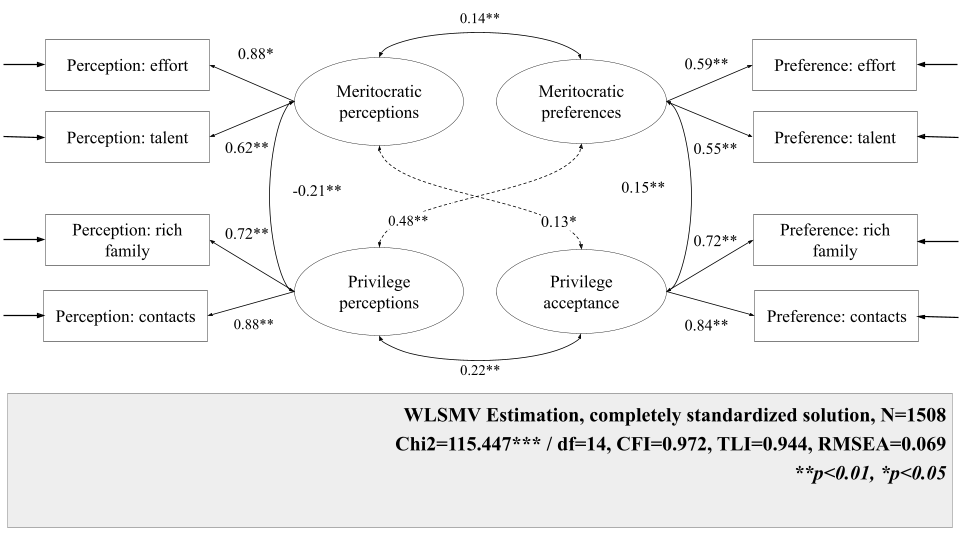
\includegraphics[width=1\linewidth,height=\textheight,keepaspectratio]{../paper/imagenes/esquema-general.png}

}

\end{figure}%

All standardized factor loadings are statistically significant and
generally moderate to strong, though their magnitude varies across
dimensions. For meritocratic perceptions, both indicators load
positively on the latent factor, with effort showing a particularly
strong loading (\(\beta\) = 0.88) and talent a moderately strong loading
(\(\beta\) = 0.62). Meritocratic preferences exhibit more even, but
somewhat weaker, loadings for effort (\(\beta\) = 0.59) and talent
(\(\beta\) = 0.55). For perceived privilege, both indicators load
strongly, especially contacts (\(\beta\) = 0.88), followed by coming
from a rich family (\(\beta\) = 0.72). Privilege acceptance also shows
strong and relatively balanced loadings, with contacts (\(\beta\) =
0.84) and rich family (\(\beta\) = 0.72), indicating that both
indicators are similarly representative of this latent dimension.

The latent correlations reveal a differentiated structure among the four
dimensions. Meritocratic perceptions and meritocratic preferences are
positively correlated (\(r\) = 0.14), consistent with some alignment
between what students perceive is rewarded and what they believe should
be rewarded. Meritocratic perceptions and privilege perceptions are
negatively correlated (\(r\) = −0.21), suggesting that students who
perceive greater meritocracy in society tend to view a weaker role for
connections and family wealth. At the same time, privilege perceptions
are positively related to meritocratic preferences (\(r\) = 0.48,
strongest correlation), suggesting that perceiving society as rewarding
contacts and wealth may coincide with stronger endorsement of
meritocratic ideals. Finally, meritocratic preferences and privilege
acceptance are modestly positively correlated (\(r\) = 0.15), and
privilege perceptions and preferences are also positively associated
(\(r\) = 0.22), indicating that recognizing privilege in practice is
linked to a greater acceptance of their legitimacy, albeit to a moderate
extent.

\subsection{Invariance analysis}\label{invariance-analysis}

\subsubsection{Longitudinal invariance}\label{longitudinal-invariance}

Figure~\ref{fig-likerplot1} displays the response distributions for the
meritocracy scale, distinguishing perceptions (Panel A) from preferences
(Panel B) across waves. Across both waves, a clear and stable gap
emerges between how students perceive social rewards to operate and how
they think they should operate. In the perception items, agreement is
consistently high for contacts, parental wealth, and talent, whereas
effort is also widely endorsed but to a lesser extent, indicating that
students recognize both meritocratic and privilege determinants of
success and view talent as more influential than effort. In the
preference items, by contrast, effort is overwhelmingly endorsed as the
legitimate basis for rewards, far exceeding its perceived role in
practice. Talent occupies a more ambivalent normative position, parental
wealth remains evenly divided, and contacts are more often accepted than
rejected, suggesting that privilege criteria are not uniformly seen as
illegitimate. Wave 2 closely replicates these patterns, with only modest
shifts. Overall, the descriptive results reveal a persistent paradox:
strong endorsement of effort-centered meritocratic ideals alongside
skepticism about their realization in practice.

\begin{figure}

\caption{\label{fig-likerplot1}Distribution of responses on the scale of
perceptions and preferences regarding meritocracy by wave}

\centering{


\includegraphics[width=1\linewidth,height=\textheight,keepaspectratio]{paper_blinded_files/figure-pdf/fig-likerplot1-1.pdf}

}

\end{figure}%

Table~\ref{tbl-longinv} reports the results of the longitudinal
invariance tests. Overall, the scale achieved the strongest level of
invariance (strict invariance) across the two waves. The strict model
showed good fit, \(\chi^2\)(84) = 130.17, CFI = 0.991, RMSEA = 0.031
(90\% CI: 0.020--0.040). Moreover, compared with the strong (scalar)
model, the deterioration in fit was negligible: \(\Delta \chi^2\)(4) =
1.635, \(\Delta\)CFI = 0.000, and \(\Delta\)RMSEA = -0.002. These
differences fall well within commonly used cutoffs for invariance
evaluation (\citeproc{ref-chen_sensitivity_2007}{Chen, 2007}),
indicating that constraining residual variances in addition to loadings
and thresholds/intercepts is tenable. Substantively, this implies that
the item--factor relations are stable over time (metric invariance) and
that, for a given level of the latent trait, respondents are expected to
endorse the same response categories across waves (scalar invariance),
supporting the comparability of scores and latent parameters within
students over time.

\begin{table}[H]

\caption{\label{tbl-longinv}Longitudinal invariance results}

\centering{

\centering\begingroup\fontsize{9.5}{11.5}\selectfont

\resizebox{\ifdim\width>\linewidth\linewidth\else\width\fi}{!}{
\begin{tabular}{>{\centering\arraybackslash}p{2cm}>{\centering\arraybackslash}p{2.1cm}>{\centering\arraybackslash}p{1.3cm}>{\centering\arraybackslash}p{2.2cm}>{\centering\arraybackslash}p{2.4cm}>{\centering\arraybackslash}p{1.3cm}>{\centering\arraybackslash}p{1.4cm}>{\centering\arraybackslash}p{2cm}}
\toprule
Model & $\chi^2$ (df) & CFI & RMSEA (90\% CI) & $\Delta \chi^2$ ($\Delta$df) & $\Delta$CFI & $\Delta$RMSEA & Decision\\
\midrule
Configural & 117.7 (68) & 0.991 & 0.035 
 (0.024-0.046) & 0 (0) & 0 & 0.000 & Reference\\
Weak & 122.51 (72) & 0.990 & 0.034 
 (0.024-0.045) & 4.809 (4) & 0 & -0.001 & Accept\\
Strong & 128.53 (80) & 0.991 & 0.032 
 (0.021-0.042) & 6.02 (8) & 0 & -0.002 & Accept\\
Strict & 130.17 (84) & 0.991 & 0.031 
 (0.02-0.04) & 1.635 (4) & 0 & -0.002 & Accept\\
\bottomrule
\end{tabular}}
\endgroup{}

}

\end{table}%

As an additional diagnostic, we used univariate score tests to identify
potential sources of localized misfit at each step of the invariance
hierarchy. The tests revealed no meaningful violations of the imposed
equality constraints, suggesting that model fit was not driven by a
small subset of parameters. Global score tests and the smallest p-values
at each step are reported in the Supplementary Material.

\subsubsection{Cohort invariance}\label{cohort-invariance}

Figure~\ref{fig-likerplot2} shows response distributions by cohort,
separating perceptions and preferences. In primary education, effort and
talent are perceived as similarly rewarded, while contacts and family
wealth are also seen as advantageous, though with more disagreement. In
secondary education, perceptions become less meritocratic: agreement
that effort is rewarded declines, whereas contacts and family wealth are
seen as more strongly shaping success. Preferences are more stable
across cohorts. In both groups, effort is the most strongly endorsed
legitimate basis for reward, while talent, family wealth, and especially
contacts remain more ambivalent. Notably, contacts are more often
accepted than rejected in both cohorts. Overall, the cohort comparison
reveals a widening gap between an effort-centered meritocratic ideal and
the perceived importance of privilege advantages in practice.

\begin{figure}

\caption{\label{fig-likerplot2}Distribution of responses on the scale of
perceptions and preferences regarding meritocracy by cohort}

\centering{


\includegraphics[width=1\linewidth,height=\textheight,keepaspectratio]{paper_blinded_files/figure-pdf/fig-likerplot2-1.pdf}

}

\end{figure}%

\begin{table}[H]

\caption{\label{tbl-cohort2}Cohort (multigroup) invariance results}

\centering{

\centering\begingroup\fontsize{9.5}{11.5}\selectfont

\resizebox{\ifdim\width>\linewidth\linewidth\else\width\fi}{!}{
\begin{tabular}{>{\centering\arraybackslash}p{2.6cm}>{\centering\arraybackslash}p{2cm}>{\centering\arraybackslash}p{1.3cm}>{\centering\arraybackslash}p{2.2cm}>{\centering\arraybackslash}p{2.3cm}>{\centering\arraybackslash}p{1.3cm}>{\centering\arraybackslash}p{1.3cm}>{\centering\arraybackslash}p{1.7cm}}
\toprule
Model & $\chi^2$ (df) & CFI & RMSEA (90\% CI) & $\Delta \chi^2$ ($\Delta$df) & $\Delta$CFI & $\Delta$RMSEA & Decision\\
\midrule
Configural & 24.95 (26) & 0.993 & 0.036 
(0.009-0.057) & 0 (0) & 0.000 & 0.000 & Reference\\
Tresholds & 57.56 (42) & 0.980 & 0.049 
(0.033-0.064) & 43.875 (16) *** & -0.013 & 0.013 & Reject\\
Tresholds + Loadings & 72.35 (46) & 0.973 & 0.053 
(0.039-0.067) & 17.075 (4) ** & -0.006 & 0.005 & Reject\\
\bottomrule
\end{tabular}}
\endgroup{}

}

\end{table}%

Table~\ref{tbl-cohort2} summarizes the cross-cohort invariance tests.
The scale achieves configural invariance between primary and secondary
students, but not threshold invariance, and therefore does not meet the
prerequisites for stronger forms of invariance
(\citeproc{ref-svetina_multiplegroup_2020}{Svetina et al., 2020};
\citeproc{ref-wu_identification_2016a}{Wu \& Estabrook, 2016}).
Constraining thresholds worsened model fit (\(\Delta\)CFI = −.013;
\(\Delta\)RMSEA = .013), exceeding recommended cutoffs
(\citeproc{ref-chen_sensitivity_2007}{Chen, 2007}). This indicates that
response categories do not map equivalently onto the latent constructs
across cohorts, limiting direct comparisons of latent means or other
latent differences.

To locate the source of cross-cohort non-invariance, we inspected
localized misfit in the threshold-invariant model. The largest
violations concerned the perceived-effort item, especially the second
threshold (\(\chi^2=10.12, p=.001\)) and, to a lesser extent, the first
(\(\chi^2=7.55, p=.006\)), suggesting that older students may apply a
more critical standard when judging whether effort is rewarded in
society.

Despite the lack of cohort invariance, re-estimating the longitudinal
invariance models with cohort as a covariate predicting each latent
factor did not materially change model fit or conclusions, suggesting
that invariance over time remains tenable. These robustness checks are
reported in the Supplementary Material.

\section{Discussion}\label{discussion}

The first hypothesis proposed that students' meritocratic beliefs would
be best represented by four distinct factors: perceived meritocracy,
perceived privilege, meritocratic preferences, and privilege acceptance.
The confirmatory factor analyses support this expectation: the scale
performs well in the school-aged population, with satisfactory model
fit, strong factor loadings, and meaningful correlations among factors.
Consistent with evidence from adult populations
(\citeproc{ref-castillo_multidimensional_2023}{Castillo et al., 2023}),
these results indicate that even at an early stage of school
socialization, students distinguish between perceptions and preferences,
and between meritocratic and privilege-based principles. This
four-factor structure also resonates with qualitative evidence from
Chilean schools, where students across socioeconomic groups
simultaneously invoke meritocratic ideals and recognize structural
advantage (\citeproc{ref-neutaguayo_neoliberalism_2025}{Neut Aguayo et
al., 2025}), and where merit is often defined by attitude and visible
effort rather than by academic outcomes
(\citeproc{ref-moyanodavila_merit_2025}{Moyano Dávila et al., 2025}).
This last finding is relevant for interpreting the privilege acceptance
dimension: in contexts where merit is primarily understood as behavioral
disposition, accepting that privilege-based advantages lead to better
outcomes may not be experienced as a contradiction but as a separate
normative judgment about a different domain, a reading that, while going
beyond what Moyano Dávila et al.
(\citeproc{ref-moyanodavila_merit_2025}{2025}) directly establish, is
consistent with their evidence. This suggests that the coexistence of
these orientations reflects how students actually navigate competing
narratives about fairness and reward, rather than an artifact of survey
design.

The empirical separability of these dimensions has substantive
implications for how meritocratic beliefs are understood and measured
(\citeproc{ref-kwon_multidimensionality_2024}{Kwon \& Pandian, 2024};
\citeproc{ref-mijs_visualizing_2026}{Mijs, 2026};
\citeproc{ref-zhu_meritocratic_2025}{Zhu, 2025}). Perceived and
preferred meritocracy are already distinguishable among school-aged
students, consistent with the distinction between ``what is'' and ``what
should be'' and with earlier attempts to operationalize it
(\citeproc{ref-castillo_multidimensional_2023}{Castillo et al., 2023};
\citeproc{ref-duru-bellat_whos_2012}{Duru-Bellat \& Tenret, 2012}). This
matters because the same normative endorsement of merit can carry
different meanings depending on perceived reality: high perceived
meritocracy is more compatible with affirming existing arrangements,
whereas low perceived meritocracy can reflect dissatisfaction and a
demand for greater fairness. At the same time, meritocratic and
privilege-based principles coexist rather than forming opposite poles of
a single continuum, directly challenging zero-sum measurement strategies
that presuppose endorsing merit entails rejecting privilege
(\citeproc{ref-reynolds_perceptions_2014a}{Reynolds \& Xian, 2014};
\citeproc{ref-wiesner_effort_2026}{Wiesner \& Sachweh, 2026}). The
correlational pattern in our data reinforces this: perceived privilege
is positively associated with stronger meritocratic preferences,
suggesting a normative-reactive response to perceived unfairness
(\citeproc{ref-castillo_multidimensional_2023}{Castillo et al., 2023}).
This is consistent with Zhu's
(\citeproc{ref-zhu_meritocratic_2025}{2025}) argument that meritocratic
and structural explanations accumulate rather than displace one another,
and with accounts in which merit endorsement may remain stable as
recognition of structural constraints increases
(\citeproc{ref-liu_does_2025}{C. Liu \& Wang, 2025};
\citeproc{ref-tang_meritocratic_2025}{Tang et al., 2025}). It is also
worth noting how this finding relates to typological approaches: Kwon \&
Pandian (\citeproc{ref-kwon_multidimensionality_2024}{2024}) document
three distinct attitudinal clusters in Europe, showing that coexistence
takes different forms across individuals. The present study complements
that work by showing how the same coexistence can be represented within
a single coherent measurement model that supports longitudinal
inference, rather than requiring person-centered classification. This
has concrete implications for how educators and policy designers
interpret students' orientations toward fairness. A student who strongly
endorses merit as an ideal while recognizing that privilege shapes
outcomes is not disengaged or fatalistic: they hold a normative demand
for fairness that the system is not meeting. Conflating this profile
with one of simple disbelief in effort leads to misdiagnosis, whether in
classroom practice or in policy design. Distinguishing which dimension
is at stake, endorsement of merit, recognition of privilege, or
acceptance of it as legitimate, matters for how schools interpret
students' sense of fairness and respond to it through civic education,
classroom climate, and efforts to build trust in the fairness of school
itself.

These results also have implications for how the existing literature on
school meritocracy should be interpreted. A substantial body of research
has linked stronger meritocratic beliefs among students to inequality
legitimation, weaker support for redistribution, and greater acceptance
of unequal access to educational resources
(\citeproc{ref-batruch_belief_2022}{Batruch et al., 2022};
\citeproc{ref-castillo_socialization_2024}{Castillo et al., 2024};
\citeproc{ref-wiederkehr_belief_2015}{Wiederkehr et al., 2015}), while
among teachers and parents, similar beliefs predict competitive
classroom practices and lower demand for equity-oriented policies
(\citeproc{ref-darnon_competitive_2023}{Darnon et al., 2023}). A
particularly relevant finding is that perceived, but not preferred,
school meritocracy predicts lower support for egalitarian and inclusive
educational interventions (\citeproc{ref-darnon_belief_2018}{Darnon,
Smeding, et al., 2018}), and that belief in school meritocracy is
associated with greater acceptance of social-class achievement gaps
(\citeproc{ref-darnon_where_2018}{Darnon, Wiederkehr, et al., 2018}).
However, most of this research relies on unidimensional or
undifferentiated measures, which means it cannot establish whether these
effects are specific to particular dimensions or reflect a more general
meritocratic orientation. Our findings suggest that these documented
effects are likely dimension-specific: perceived meritocracy is not
equivalent to preferred meritocracy, and neither carries the same
consequences as perceived privilege or privilege acceptance. The
contrast with Chauvin et al. (\citeproc{ref-chauvin_school_2026}{2026})
is instructive here, as theirs is the closest existing instrument: by
distinguishing ability and equity within a bifactor model, they
establish that school meritocracy is multidimensional, but because their
measure is confined to teachers and to perceived meritocracy, it cannot
speak to whether students separate what they perceive from what they
prefer, or merit from privilege. What the present study adds is a
four-factor structure validated in students and shown to be
longitudinally invariant, which provides the measurement foundation
needed to examine whether distinct dimensions of meritocratic belief
carry distinct consequences for the educational environment, from
students' sense of justice in school to civic attitudes and the broader
climate of fairness, a question the existing literature has not yet been
able to address with adequate precision.

The second hypothesis stated that the measurement model would be stable
over time, and the results support this expectation. Achieving strict
longitudinal invariance indicates that the scale functions equivalently
across waves, measuring the same latent constructs at each time point.
This is crucial in developmental research because without invariance,
apparent change may reflect shifts in how students interpret items or
use response categories rather than genuine change in underlying beliefs
(\citeproc{ref-liu_testing_2017}{Y. Liu et al., 2017};
\citeproc{ref-putnick_measurement_2016}{Putnick \& Bornstein, 2016};
\citeproc{ref-vandeschoot_editorial_2015}{Van De Schoot et al., 2015}).
With strict invariance in place, observed differences over time can be
interpreted as substantive within-student change rather than measurement
artifact, strengthening longitudinal inference and supporting models
such as latent mean comparisons or growth curve analyses
(\citeproc{ref-putnick_measurement_2016}{Putnick \& Bornstein, 2016}).
Substantively, the results suggest that meritocratic belief structures
are relatively stable over a one-year window in early-to-mid
adolescence, which has implications for when educational interventions
targeting these beliefs are likely to produce measurable change. This
longitudinal invariance also provides the measurement foundation for
subsequent studies to examine how distinct dimensions of meritocratic
belief relate to outcomes such as academic motivation, civic attitudes,
and school well-being. In this regard, Liu \& Wang's
(\citeproc{ref-liu_does_2025}{2025}) distinction between education
operating as legitimation or as enlightenment, depending on the broader
inequality context, points to a productive direction: whether perceived
privilege leads to stronger meritocratic preferences or to disengagement
from institutional narratives may depend on the degree to which the
educational system is experienced as fair, a question that requires
dimensionally validated instruments to examine adequately.

The third hypothesis proposed invariance across educational levels. The
results did not support full metric or scalar equivalence:
non-invariance is concentrated in perceived meritocracy, specifically in
how students at different school stages interpret whether effort is
rewarded in society. Rather than treating this as a measurement failure,
we interpret it as a substantive theoretical finding. Cross-cohort
non-invariance indicates that primary and secondary students do not
merely differ in their level of perceived meritocracy: they attach
qualitatively different meanings to the concept of effort being
rewarded. This is consistent with developmental research showing that
adolescence is precisely the period when abstract reasoning about
justice and fairness becomes more sophisticated and when school-based
sorting mechanisms, including grades, tracking, and peer comparison,
grow increasingly salient (\citeproc{ref-henry_development_2006}{Henry
\& Saul, 2006}; \citeproc{ref-resh_sense_2014}{Resh \& Sabbagh, 2014}),
providing students with a richer and more critical experiential basis
for evaluating meritocratic claims. A plausible mechanism is that
cumulative exposure to these processes produces a progressive reality
shock (\citeproc{ref-allen_top_2016}{Allen, 2016};
\citeproc{ref-tang_meritocratic_2025}{Tang et al., 2025}), such that
older students evaluate the same item through a more critical and
experience-laden lens. If the SES-differentiated convergence documented
by Tang et al. (\citeproc{ref-tang_meritocratic_2025}{2025}) operates
earlier, during secondary school in Chile's highly stratified system,
the non-invariance concentrated in the perceived-effort item may partly
reflect students across social positions increasingly confronting the
limits of effort as a sufficient explanation for outcomes. In Chile's
highly stratified system, where the gap between meritocratic discourse
and structural reality is particularly visible, students from lower
socioeconomic backgrounds have been shown to experience this gap as a
moral grievance (\citeproc{ref-neutaguayo_neoliberalism_2025}{Neut
Aguayo et al., 2025}), which is consistent with the idea that the
construct of perceived effort becomes more contested, and therefore less
stable across students, as schooling advances. For researchers, this is
a call to move beyond assuming that meritocracy scales travel unchanged
across school levels: future work should prioritize stage-sensitive item
formulations and partial invariance approaches that can accommodate
meaning shifts without sacrificing cross-level comparability
(\citeproc{ref-putnick_measurement_2016}{Putnick \& Bornstein, 2016};
\citeproc{ref-vandeschoot_checklist_2012}{Van De Schoot et al., 2012}).
For practitioners, including teachers and those designing civic
education and school-climate initiatives, the finding indicates that the
same meritocratic message may be processed through different
interpretive frames depending on students' accumulated school
experience, and that efforts to foster a shared sense of fairness in
school need to be calibrated to developmental stage rather than applied
uniformly across grade levels.

Taken together, the longitudinal and cross-cohort findings are not
contradictory but jointly informative. Longitudinal invariance was
established within the same students over a one-year window: within that
period, the scale measures the same constructs in the same way, and
observed change can be interpreted as substantive. Cross-cohort
non-invariance reflects a different comparison, two groups separated by
approximately two to three years of accumulated schooling, and points to
a longer developmental process through which cumulative school
experience progressively reshapes how students interpret whether effort
is rewarded. The instrument is therefore well-suited for longitudinal
inference within the same school stage, while cross-stage comparisons
require caution and, ideally, stage-sensitive measurement approaches.

\section{Conclusion}\label{conclusion}

Schools socialize students into beliefs about meritocracy, promoting
effort and talent as the legitimate basis of reward while simultaneously
exposing students to the weight of family resources and social
connections in shaping outcomes
(\citeproc{ref-goudeau_hidden_2017a}{Goudeau \& Croizet, 2017};
\citeproc{ref-resh_sense_2014}{Resh \& Sabbagh, 2014};
\citeproc{ref-traini_stratification_2022}{Traini, 2022}). Students
navigate this tension by holding both orientations at once, endorsing
merit as an ideal while recognizing that privilege structures actual
outcomes, a configuration the literature describes as dual consciousness
(\citeproc{ref-liu_does_2025}{C. Liu \& Wang, 2025};
\citeproc{ref-tang_meritocratic_2025}{Tang et al., 2025}). Capturing
this complexity requires instruments that distinguish how students
perceive meritocracy to work from how they prefer it should work, and
that treat merit and privilege as potentially coexisting rather than
mutually exclusive, a standard most available measures do not meet.
Extending Castillo et al.'s
(\citeproc{ref-castillo_multidimensional_2023}{2023}) multidimensional
framework to adolescents, this study tests whether students distinguish
merit from privilege and perceptions (``what is'') from preferences
(``what should be''), using panel survey data from two Chilean cohorts
(8th and 10th graders) across two waves (2023-2024), and whether these
dimensions are stable over time and comparable across school stages. The
contribution is a modest but foundational one: to establish whether
meritocratic beliefs can be measured reliably and equivalently in
school-aged populations, as a precondition for studying their
developmental trajectory and educational consequences.

The results support a four-factor structure, perceived meritocracy,
perceived privilege, meritocratic preferences, and privilege acceptance,
showing that Chilean adolescents differentiate perceptions from
preferences and meritocratic from privilege-based principles, and that
merit endorsement can coexist with recognition of structural advantage.
Consistent with this, perceived privilege is positively associated with
stronger meritocratic preferences, suggesting that recognizing unfair
advantages can intensify demands that rewards should follow merit, a
normative-reactive pattern that unidimensional instruments would obscure
(\citeproc{ref-castillo_multidimensional_2023}{Castillo et al., 2023};
\citeproc{ref-mijs_visualizing_2026}{Mijs, 2026};
\citeproc{ref-wiesner_effort_2026}{Wiesner \& Sachweh, 2026}). The
measurement structure is longitudinally invariant within students,
providing a reliable basis for interpreting over-time change as
substantive rather than artifactual. At the same time, cross-cohort
non-invariance is itself a substantive finding rather than merely a
technical caveat: comparisons across educational stages require caution
because the perception that ``effort is rewarded'' does not carry the
same meaning for primary and secondary students. This measurement
heterogeneity is theoretically consistent with developmental accounts in
which cumulative schooling experience progressively reshapes how
students interpret meritocratic signals
(\citeproc{ref-allen_top_2016}{Allen, 2016};
\citeproc{ref-tang_meritocratic_2025}{Tang et al., 2025}), and it calls
for stage-sensitive item formulations in future work rather than
treating the current scale as directly comparable across levels. In
doing so, the instrument moves beyond the most recent dedicated
alternative, the teacher-focused, perception-only scale of Chauvin et
al. (\citeproc{ref-chauvin_school_2026}{2026}), toward a measure that
captures how students themselves distinguish merit from privilege and
description from preference.

More broadly, these findings sharpen how the literature should interpret
meritocracy effects in educational contexts. By distinguishing
dimensions that unidimensional measures collapse, the four-factor model
shows that part of what is often read as a decline in belief in
meritocracy may instead reflect growing recognition of structural
constraints rather than weaker merit endorsement
(\citeproc{ref-liu_does_2025}{C. Liu \& Wang, 2025};
\citeproc{ref-reynolds_perceptions_2014a}{Reynolds \& Xian, 2014};
\citeproc{ref-tang_meritocratic_2025}{Tang et al., 2025};
\citeproc{ref-zhu_meritocratic_2025}{Zhu, 2025}). It also offers a
distinct route to the coexistence of contrasting beliefs: where
typological approaches document that coexistence by sorting individuals
into attitudinal clusters
(\citeproc{ref-kwon_multidimensionality_2024}{Kwon \& Pandian, 2024};
\citeproc{ref-zhu_meritocratic_2025}{Zhu, 2025}), the present study
represents it within a single measurement model that supports
longitudinal inference, rather than requiring person-centered
classification. The combination of strict longitudinal invariance and
cross-level non-invariance establishes a key boundary condition:
within-student comparisons over time are warranted, whereas comparisons
across school stages must account for the shifting meaning of perceived
meritocracy.

Although this study draws on a single country, its contributions carry
implications beyond the Chilean case. Three findings are likely to
travel across educational systems. First, the conceptual distinction
between perceived and preferred meritocracy, and between meritocratic
and privilege-based principles, reflects general cognitive and normative
capacities that develop during adolescence regardless of national
context; the four-factor structure should therefore replicate in other
highly stratified systems. Second, the coexistence of merit endorsement
and recognition of privilege, the core pattern underlying dual
consciousness, has been documented in China
(\citeproc{ref-liu_does_2025}{C. Liu \& Wang, 2025};
\citeproc{ref-tang_meritocratic_2025}{Tang et al., 2025}), the United
States and Finland (\citeproc{ref-zhu_meritocratic_2025}{Zhu, 2025}),
and Europe (\citeproc{ref-kwon_multidimensionality_2024}{Kwon \&
Pandian, 2024}), suggesting it is not a Chilean peculiarity. Third, the
logic of longitudinal invariance testing as a prerequisite for
developmental inference is methodologically general and applies to any
panel study of meritocratic beliefs. By contrast, the specific pattern
of cross-cohort non-invariance, concentrated in perceived effort, may be
more system-dependent: it likely reflects the particular intensity and
timing of school-based sorting in Chile's tracked and marketized system.
Future research in countries with different tracking regimes and
stratification profiles will help clarify which aspects of measurement
equivalence are universal and which are conditioned by institutional
features.

The findings carry distinct implications for three audiences. For
researchers, the results underscore the importance of treating
meritocratic beliefs as multidimensional and of testing measurement
invariance before making developmental or cross-group comparisons, since
otherwise observed differences may reflect differential item
interpretation rather than genuine attitudinal divergence, particularly
across socioeconomic or generational groups. For practitioners,
including teachers, school counselors, and those who design civic and
citizenship education, the coexistence of merit endorsement and
recognition of privilege suggests that students are not passive
recipients of meritocratic ideals but actively navigate tensions between
what schools tell them about fairness and what they observe in practice.
This has direct relevance for civic education and for school climate:
rather than simply reinforcing effort-based narratives or, conversely,
dismantling them, educators can engage students' existing dual awareness
as a starting point for discussing how merit and privilege coexist,
helping cultivate a more critical and grounded sense of justice. Because
the meanings students attach to effort and reward shift across school
stages, such efforts need to be calibrated to students' developmental
moment rather than applied uniformly. For policymakers concerned with
equity, the finding that perceived privilege intensifies meritocratic
preferences carries a specific message: students who recognize that
rewards do not follow merit do not abandon the ideal of fairness but
demand it more strongly. Educational systems that maintain a strong
meritocratic discourse while visibly reproducing inequality risk
widening the gap between what they promise and what students experience,
with potential consequences for students' sense of justice in school,
their trust in educational institutions, and their broader civic
engagement.

This study has limitations that point to clear directions for future
research. The scale is deliberately minimalist, with two items per
factor, which constrains content coverage and reliability and means that
claims about subtle within-dimension differences should be treated with
caution. Future work should expand and refine the item pool, adding at
least one additional indicator per factor and testing whether richer
item sets alter the invariance conclusions reported here. With only two
waves and two school levels, additional waves and broader age coverage
are needed to better trace developmental trajectories and identify when
shifts in meaning in perceived meritocracy occur. Cross-level
non-invariance calls for differential item functioning analyses and
stage-sensitive item formulations to support comparability across
educational stages. Most importantly, future research should examine how
perceptions and preferences of meritocratic and privilege-based
principles relate to the outcomes for which they are most likely to
matter in school: students' sense of justice and fairness, civic
attitudes and engagement, school climate, and wellbeing, alongside
academic motivation. By providing an empirically supported and
longitudinally invariant multidimensional measure for adolescents, this
study offers a more reliable foundation for studying how school-based
meritocratic socialization shapes students' interpretations of fairness
and inequality.

\section{Declaration of generative AI and AI-assisted technologies in
the writing
process}\label{declaration-of-generative-ai-and-ai-assisted-technologies-in-the-writing-process}

During the preparation of this work, the authors used Claude (Anthropic)
to assist with language editing, restructuring, and condensing of the
manuscript text. After using this tool, the authors reviewed and edited
the content as needed and take full responsibility for the content of
the published article.

\section{References}\label{references}

\phantomsection\label{refs}
\begin{CSLReferences}{1}{0}
\bibitem[\citeproctext]{ref-allen_top_2016}
Allen, K. (2016). Top girls navigating austere times: Interrogating
youth transitions since the {``crisis.''} \emph{Journal of Youth
Studies}, \emph{19}(6), 805--820.
\url{https://doi.org/10.1080/13676261.2015.1112885}

\bibitem[\citeproctext]{ref-batruch_belief_2022}
Batruch, A., Jetten, J., Van de Werfhorst, H., Darnon, C., \& Butera, F.
(2022). Belief in {School Meritocracy} and the {Legitimization} of
{Social} and {Income Inequality}. \emph{Social Psychological and
Personality Science}, 194855062211110.
\url{https://doi.org/10.1177/19485506221111017}

\bibitem[\citeproctext]{ref-bell_equality_1972}
Bell, D. (1972). On equality: {I}. {Meritocracy} and equality. \emph{The
Public Interest}, \emph{29}, 29--68.

\bibitem[\citeproctext]{ref-bellei_estudio_2013}
Bellei, C. (2013). El estudio de la segregación socioeconómica y
académica de la educación chilena. \emph{Estudios Pedagógicos
(Valdivia)}, \emph{39}(1), 325--345.
\url{https://doi.org/10.4067/S0718-07052013000100019}

\bibitem[\citeproctext]{ref-bourdieu_reproduction_1990}
Bourdieu, P., \& Passeron, J. C. (1990). \emph{Reproduction in
{Education}, {Society} and {Culture}} (Second Edition). Sage
Publications Ltd.

\bibitem[\citeproctext]{ref-brown_confirmatory_2015}
Brown, T. A. (2015). \emph{Confirmatory factor analysis for applied
research} (Second edition). New York London: The Guilford Press.

\bibitem[\citeproctext]{ref-busemeyer_skills_2014}
Busemeyer, M. (2014). \emph{Skills and {Inequality}: {Partisan Politics}
and the {Political Economy} of {Education Reforms} in {Western Welfare
States}}. Cambridge University Press.

\bibitem[\citeproctext]{ref-cabalin_framing_2023}
Cabalin, C., Saldaña, M., \& Fernández, M. B. (2023). Framing school
choice and merit: News media coverage of an education policy in {Chile}.
\emph{Discourse: Studies in the Cultural Politics of Education},
\emph{44}(6), 927--942.
\url{https://doi.org/10.1080/01596306.2023.2218272}

\bibitem[\citeproctext]{ref-castillo_multidimensional_2023}
Castillo, J. C., Iturra, J., Maldonado, L., Atria, J., \& Meneses, F.
(2023). A {Multidimensional Approach} for {Measuring Meritocratic
Beliefs}: {Advantages}, {Limitations} and {Alternatives} to the {ISSP
Social Inequality Survey}. \emph{International Journal of Sociology},
\emph{53}(6), 448--472.
\url{https://doi.org/10.1080/00207659.2023.2274712}

\bibitem[\citeproctext]{ref-castillo_perceptions_2025}
Castillo, J. C., Laffert, A., Carrasco, K., \& Iturra-Sanhueza, J.
(2025). Perceptions of inequality and meritocracy: Their interplay in
shaping preferences for market justice in {Chile} (2016--2023).
\emph{Frontiers in Sociology}, \emph{10}, 1634219.
\url{https://doi.org/10.3389/fsoc.2025.1634219}

\bibitem[\citeproctext]{ref-castillo_socialization_2024}
Castillo, J. C., Salgado, M., Carrasco, K., \& Laffert, A. (2024). The
{Socialization} of {Meritocracy} and {Market Justice Preferences} at
{School}. \emph{Societies}, \emph{14}(11), 214.
\url{https://doi.org/10.3390/soc14110214}

\bibitem[\citeproctext]{ref-castillo_meritocracia_2019}
Castillo, J. C., Torres, A., Atria, J., \& Maldonado, L. (2019).
Meritocracia y desigualdad económica: {Percepciones}, preferencias e
implicancias. \emph{Revista Internacional de Sociología}, \emph{77}(1),
117. \url{https://doi.org/10.3989/ris.2019.77.1.17.114}

\bibitem[\citeproctext]{ref-chauvin_school_2026}
Chauvin, B., Rauscher, C., Saidah, B., \& Louvet, E. (2026). School
meritocracy: A multidimensional construct? {Evidence} from the
development of a school meritocracy scale by exploratory and
confirmatory bifactor modeling. \emph{Current Psychology}, \emph{45}(5),
519. \url{https://doi.org/10.1007/s12144-026-09134-1}

\bibitem[\citeproctext]{ref-chen_sensitivity_2007}
Chen, F. F. (2007). Sensitivity of {Goodness} of {Fit Indexes} to {Lack}
of {Measurement Invariance}. \emph{Structural Equation Modeling: A
Multidisciplinary Journal}, \emph{14}(3), 464--504.
\url{https://doi.org/10.1080/10705510701301834}

\bibitem[\citeproctext]{ref-darnon_competitive_2023}
Darnon, C., Jury, M., Goudeau, S., \& Portex, M. (2023). Competitive and
cooperative practices in education: {How} teachers' beliefs in school
meritocracy are related to their daily practices with students.
\emph{Social Psychology of Education}, \emph{26}(6), 1789--1805.
\url{https://doi.org/10.1007/s11218-023-09824-9}

\bibitem[\citeproctext]{ref-darnon_belief_2018}
Darnon, C., Smeding, A., \& Redersdorff, S. (2018). Belief in school
meritocracy as an ideological barrier to the promotion of equality.
\emph{European Journal of Social Psychology}, \emph{48}(4), 523--534.
\url{https://doi.org/10.1002/ejsp.2347}

\bibitem[\citeproctext]{ref-darnon_where_2018}
Darnon, C., Wiederkehr, V., Dompnier, B., \& Martinot, D. (2018).
{``{Where} there is a will, there is a way''}: {Belief} in school
meritocracy and the social-class achievement gap. \emph{British Journal
of Social Psychology}, \emph{57}(1), 250--262.
\url{https://doi.org/10.1111/bjso.12214}

\bibitem[\citeproctext]{ref-day_movin_2017}
Day, M. V., \& Fiske, S. T. (2017). Movin' on {Up}? {How Perceptions} of
{Social Mobility Affect Our Willingness} to {Defend} the {System}.
\emph{Social Psychological and Personality Science}, \emph{8}(3),
267--274. \url{https://doi.org/10.1177/1948550616678454}

\bibitem[\citeproctext]{ref-deng_its_2025}
Deng, Y., \& Wang, F. (2025). It's my fault, {I} should try harder!
{The} narratives of self-made upward mobility sustain belief in
meritocracy in low social mobility context. \emph{British Journal of
Psychology}, bjop.70015. \url{https://doi.org/10.1111/bjop.70015}

\bibitem[\citeproctext]{ref-duru-bellat_whos_2012}
Duru-Bellat, M., \& Tenret, E. (2012). Who's for {Meritocracy}?
{Individual} and {Contextual Variations} in the {Faith}.
\emph{Comparative Education Review}, \emph{56}(2), 223--247.
\url{https://doi.org/10.1086/661290}

\bibitem[\citeproctext]{ref-fercovic_disentangling_2022}
Fercovic, M. (2022). Disentangling {Meritocracy Among} the {Long-Range
Upwardly Mobile}: {The Chilean Case}. \emph{Sociological Research
Online}, \emph{27}(1), 118--135.
\url{https://doi.org/10.1177/1360780420963395}

\bibitem[\citeproctext]{ref-ferre_welfare_2023}
Ferre, J. C. (2023). Welfare regimes in twenty-first-century {Latin
America}. \emph{Journal of International and Comparative Social Policy},
\emph{39}(2), 101--127. \url{https://doi.org/10.1017/ics.2023.16}

\bibitem[\citeproctext]{ref-garcia-sierra_dark_2023}
García-Sierra, A. (2023). The dark side of meritocratic beliefs: {Is}
believing in meritocracy detrimental to individuals from low
socioeconomic backgrounds? \emph{Social Justice Research}, \emph{36}(4),
385--409. \url{https://doi.org/10.1007/s11211-023-00413-x}

\bibitem[\citeproctext]{ref-gingrich_making_2011}
Gingrich, J. R. (2011). \emph{Making {Markets} in the {Welfare State}:
{The Politics} of {Varying Market Reforms}} (1st ed.). Cambridge
University Press. \url{https://doi.org/10.1017/CBO9780511791529}

\bibitem[\citeproctext]{ref-goudeau_hidden_2017a}
Goudeau, S., \& Croizet, J.-C. (2017). Hidden {Advantages} and
{Disadvantages} of {Social Class}: {How Classroom Settings Reproduce
Social Inequality} by {Staging Unfair Comparison}. \emph{Psychological
Science}, \emph{28}(2), 162--170.
\url{https://doi.org/10.1177/0956797616676600}

\bibitem[\citeproctext]{ref-henry_development_2006}
Henry, P. J., \& Saul, A. (2006). The {Development} of {System
Justification} in the {Developing World}. \emph{Social Justice
Research}, \emph{19}(3), 365--378.
\url{https://doi.org/10.1007/s11211-006-0012-x}

\bibitem[\citeproctext]{ref-heuer_legitimizing_2020}
Heuer, J.-O., Lux, T., Mau, S., \& Zimmermann, K. (2020). Legitimizing
{Inequality}: {The Moral Repertoires} of {Meritocracy} in {Four
Countries}. \emph{Comparative Sociology}, \emph{19}(4-5), 542--584.
\url{https://doi.org/10.1163/15691330-BJA10017}

\bibitem[\citeproctext]{ref-imhoff_nociones_2025}
Imhoff, D., \& Brussino, S. (2025). {Nociones infantiles sobre
desigualdad social: atravesamientos ideológicos y procesos de
socialización política}. \emph{Revista Latinoamericana de Ciencias
Sociales, Niñez y Juventud}, \emph{13}(2).
\url{https://doi.org/10.11600/1692715x.1329071114}

\bibitem[\citeproctext]{ref-janmaat_subjective_2013}
Janmaat, J. G. (2013). Subjective {Inequality}: A {Review} of
{International Comparative Studies} on {People}'s {Views} about
{Inequality}. \emph{European Journal of Sociology}, \emph{54}(3),
357--389. \url{https://doi.org/10.1017/S0003975613000209}

\bibitem[\citeproctext]{ref-jost_decade_2004a}
Jost, J. T., Banaji, M. R., \& Nosek, B. A. (2004). A {Decade} of
{System Justification Theory}: {Accumulated Evidence} of {Conscious} and
{Unconscious Bolstering} of the {Status Quo}. \emph{Political
Psychology}, \emph{25}(6), 881--919.
\url{https://doi.org/10.1111/j.1467-9221.2004.00402.x}

\bibitem[\citeproctext]{ref-kline_principles_2023}
Kline, R. B. (2023). \emph{Principles and {Practice} of {Structural
Equation Modeling}}. Guilford Publications.

\bibitem[\citeproctext]{ref-kwon_multidimensionality_2024}
Kwon, R., \& Pandian, R. K. (2024). Multidimensionality in merit
attitudes: {The} role of hard work, skills, and social connections in
{Europe}. \emph{Social Science Research}, \emph{122}, 103056.
\url{https://doi.org/10.1016/j.ssresearch.2024.103056}

\bibitem[\citeproctext]{ref-lampert_meritocratic_2013}
Lampert, K. (2013). \emph{Meritocratic {Education} and {Social
Worthlessness}}. London: Palgrave Macmillan UK.
\url{https://doi.org/10.1057/9781137324894}

\bibitem[\citeproctext]{ref-liu_does_2025}
Liu, C., \& Wang, J. (2025). Does {Education Legitimise Inequality}?
{Comparative Analysis} of {Income Inequality}, {Education}, and
{Meritocratic Beliefs}. \emph{The British Journal of Sociology},
1468--4446.70029. \url{https://doi.org/10.1111/1468-4446.70029}

\bibitem[\citeproctext]{ref-liu_testing_2017}
Liu, Y., Millsap, R. E., West, S. G., Tein, J.-Y., Tanaka, R., \& Grimm,
K. J. (2017). Testing measurement invariance in longitudinal data with
ordered-categorical measures. \emph{Psychological Methods},
\emph{22}(3), 486--506. \url{https://doi.org/10.1037/met0000075}

\bibitem[\citeproctext]{ref-mccoy_priming_2007}
McCoy, S. K., \& Major, B. (2007). Priming meritocracy and the
psychological justification of inequality. \emph{Journal of Experimental
Social Psychology}, \emph{43}(3), 341--351.
\url{https://doi.org/10.1016/j.jesp.2006.04.009}

\bibitem[\citeproctext]{ref-mijs_unfulfillable_2016}
Mijs, J. (2016). The {Unfulfillable Promise} of {Meritocracy}: {Three
Lessons} and {Their Implications} for {Justice} in {Education}.
\emph{Social Justice Research}, \emph{29}(1), 14--34.
\url{https://doi.org/10.1007/s11211-014-0228-0}

\bibitem[\citeproctext]{ref-mijs_paradox_2021}
Mijs, J. (2021). The paradox of inequality: Income inequality and belief
in meritocracy go hand in hand. \emph{Socio-Economic Review},
\emph{19}(1), 7--35. \url{https://doi.org/10.1093/ser/mwy051}

\bibitem[\citeproctext]{ref-mijs_visualizing_2026}
Mijs, J. (2026). Visualizing {Belief} in {Merit} and {Privilege}, 1930
to 2020: {Rejoinder}. \emph{Socius: Sociological Research for a Dynamic
World}, \emph{12}, 23780231261426413.
\url{https://doi.org/10.1177/23780231261426413}

\bibitem[\citeproctext]{ref-moyanodavila_merit_2025}
Moyano Dávila, C., Alarcón-Arcos, S., Angelcos, N., Castillo, J. C., \&
Salgado, M. (2025). Merit as an {Attitude}: {Chilean School
Communities}' {Repertoires} in {Chile} and the {Perception} of the
{``{Good Student}''} in a {Post-pandemic Scenario}. \emph{Social Justice
Research}, \emph{38}(3), 264--289.
\url{https://doi.org/10.1007/s11211-025-00456-2}

\bibitem[\citeproctext]{ref-neutaguayo_neoliberalism_2025}
Neut Aguayo, P., Rivera-Vargas, P., \& Miño Puigcercós, R. (2025).
Neoliberalism and school inequality in the {Chilean} education system:
An analysis from the voices of lower-class, middle-class, and
upper-class students. \emph{International Studies in Sociology of
Education}, 1--16. \url{https://doi.org/10.1080/09620214.2025.2558938}

\bibitem[\citeproctext]{ref-oecd_trends_2025}
OECD. (2025). \emph{Trends {Shaping Education} 2025}. OECD Publishing.
\url{https://doi.org/10.1787/ee6587fd-en}

\bibitem[\citeproctext]{ref-otero_neighbourhood_2017}
Otero, G., Carranza, R., \& Contreras, D. (2017). {``{Neighbourhood}
effects''} on children's educational achievement in {Chile}: {The}
effects of inequality and polarization. \emph{Environment and Planning
A: Economy and Space}, \emph{49}(11), 2595--2618.
\url{https://doi.org/10.1177/0308518X17731780}

\bibitem[\citeproctext]{ref-putnick_measurement_2016}
Putnick, D. L., \& Bornstein, M. H. (2016). Measurement invariance
conventions and reporting: {The} state of the art and future directions
for psychological research. \emph{Developmental Review}, \emph{41},
71--90. \url{https://doi.org/10.1016/j.dr.2016.06.004}

\bibitem[\citeproctext]{ref-resh_sense_2018a}
Resh, N. (2018). Sense of {Justice} in {School} and {Social} and
{Institutional Trust}. \emph{Comparative Sociology}, \emph{17}(3-4),
369--385. \url{https://doi.org/10.1163/15691330-12341465}

\bibitem[\citeproctext]{ref-resh_sense_2014}
Resh, N., \& Sabbagh, C. (2014). Sense of justice in school and civic
attitudes. \emph{Social Psychology of Education}, \emph{17}(1), 51--72.
\url{https://doi.org/10.1007/s11218-013-9240-8}

\bibitem[\citeproctext]{ref-reynolds_perceptions_2014a}
Reynolds, J., \& Xian, H. (2014). Perceptions of meritocracy in the land
of opportunity. \emph{Research in Social Stratification and Mobility},
\emph{36}, 121--137. \url{https://doi.org/10.1016/j.rssm.2014.03.001}

\bibitem[\citeproctext]{ref-sandel_tyranny_2020}
Sandel, M. J. (2020). \emph{The tyranny of merit: {What}'s become of the
common good?} (First edition). New York: {Farrar, Straus and Giroux}.

\bibitem[\citeproctext]{ref-sigelman_age_2013a}
Sigelman, C. K. (2013). Age {Differences} in {Perceptions} of {Rich} and
{Poor People}: {Is It Skill} or {Luck}? \emph{Social Development},
\emph{22}(1), 1--18. \url{https://doi.org/10.1111/sode.12000}

\bibitem[\citeproctext]{ref-svetina_multiplegroup_2020}
Svetina, D., Rutkowski, L., \& Rutkowski, D. (2020). Multiple-{Group
Invariance} with {Categorical Outcomes Using Updated Guidelines}: {An
Illustration Using M} {\emph{plus}} and the lavaan/{semTools Packages}.
\emph{Structural Equation Modeling: A Multidisciplinary Journal},
\emph{27}(1), 111--130.
\url{https://doi.org/10.1080/10705511.2019.1602776}

\bibitem[\citeproctext]{ref-tang_meritocratic_2025}
Tang, M., Li, A., \& Wu, X. (2025). Meritocratic {Myth} in {Mind}?
{Socioeconomic Backgrounds} and {Shifting Beliefs} about {Meritocracy}
among {College Students} in {China}. \emph{Sociology of Education},
00380407251360432. \url{https://doi.org/10.1177/00380407251360432}

\bibitem[\citeproctext]{ref-tejero-peregrina_perceived_2025}
Tejero-Peregrina, L., Willis, G., Sánchez-Rodríguez, Á., \&
Rodríguez-Bailón, R. (2025). From {Perceived Economic Inequality} to
{Support} for {Redistribution}: {The Role} of {Meritocracy Perception}.
\emph{International Review of Social Psychology}, \emph{38}(1), 4.
\url{https://doi.org/10.5334/irsp.1013}

\bibitem[\citeproctext]{ref-traini_stratification_2022}
Traini, C. (2022). The stratification of education systems and social
background inequality of educational opportunity. \emph{International
Journal of Comparative Sociology}, \emph{63}(1-2), 10--29.
\url{https://doi.org/10.1177/00207152211033015}

\bibitem[\citeproctext]{ref-valenzuela_socioeconomic_2013}
Valenzuela, J. P., Bellei, C., \& Ríos, D. D. L. (2013). Socioeconomic
school segregation in a market-oriented educational system. {The} case
of {Chile}. \emph{Journal of Education Policy}, \emph{29}(2), 217--241.
\url{https://doi.org/10.1080/02680939.2013.806995}

\bibitem[\citeproctext]{ref-vandeschoot_checklist_2012}
Van De Schoot, R., Lugtig, P., \& Hox, J. (2012). A checklist for
testing measurement invariance. \emph{European Journal of Developmental
Psychology}, \emph{9}(4), 486--492.
\url{https://doi.org/10.1080/17405629.2012.686740}

\bibitem[\citeproctext]{ref-vandeschoot_editorial_2015}
Van De Schoot, R., Schmidt, P., De Beuckelaer, A., Lek, K., \&
Zondervan-Zwijnenburg, M. (2015). Editorial: {Measurement Invariance}.
\emph{Frontiers in Psychology}, \emph{6}.
\url{https://doi.org/10.3389/fpsyg.2015.01064}

\bibitem[\citeproctext]{ref-vandewerfhorst_meritocracy_2024}
Van De Werfhorst, H. G. (2024). Is {Meritocracy Not So Bad After All}?
{Educational Expansion} and {Intergenerational Mobility} in 40
{Countries}. \emph{American Sociological Review}, \emph{89}(6),
1181--1213. \url{https://doi.org/10.1177/00031224241292352}

\bibitem[\citeproctext]{ref-weinberg_countrylevel_2021}
Weinberg, D., Stevens, G. W. J. M., Currie, C., Delaruelle, K.,
Dierckens, M., Lenzi, M., \ldots{} Finkenauer, C. (2021). Country-{Level
Meritocratic Beliefs Moderate} the {Social Gradient} in {Adolescent
Mental Health}: {A Multilevel Study} in 30 {European Countries}.
\emph{Journal of Adolescent Health}, \emph{68}(3), 548--557.
\url{https://doi.org/10.1016/j.jadohealth.2020.06.031}

\bibitem[\citeproctext]{ref-wiederkehr_belief_2015}
Wiederkehr, V., Bonnot, V., Krauth-Gruber, S., \& Darnon, C. (2015).
Belief in school meritocracy as a system-justifying tool for low status
students. \emph{Frontiers in Psychology}, \emph{6}.

\bibitem[\citeproctext]{ref-wiesner_effort_2026}
Wiesner, T., \& Sachweh, P. (2026). Effort versus {Advantage}:
{Visualizing} ({Relative}) {Belief} in {Meritocracy}, 1930 to 2022---{A
Comment} on {Mijs} (2018), \emph{12}.
\url{https://doi.org/10.1177/23780231261425841}

\bibitem[\citeproctext]{ref-wu_identification_2016a}
Wu, H., \& Estabrook, R. (2016). Identification of {Confirmatory Factor
Analysis Models} of {Different Levels} of {Invariance} for {Ordered
Categorical Outcomes}. \emph{Psychometrika}, \emph{81}(4), 1014--1045.
\url{https://doi.org/10.1007/s11336-016-9506-0}

\bibitem[\citeproctext]{ref-young_rise_1958}
Young, M. (1958). \emph{The rise of the meritocracy}. New Brunswick,
N.J., U.S.A: Transaction Publishers.

\bibitem[\citeproctext]{ref-zhu_meritocratic_2025}
Zhu, L. (2025). Meritocratic beliefs in the {United States}, {Finland},
and {China}: {A} multidimensional approach using latent class analysis.
\emph{The British Journal of Sociology}, \emph{76}(1), 153--172.
\url{https://doi.org/10.1111/1468-4446.13152}

\end{CSLReferences}




\end{document}
